% !Mode:: "TeX:UTF-8"
\documentclass[11pt]{article}
\usepackage[letterpaper, margin = 2cm]{geometry}
\usepackage{microtype}
\usepackage{parskip}
\usepackage{amssymb}
\usepackage{amsmath}
\usepackage{multicol}
\usepackage{graphicx}
\usepackage{float}
\usepackage[style=ieee]{biblatex}
\usepackage[bookmarks, unicode]{hyperref}

\addbibresource{references.bib}

\title{Regen Calculations}
\author{Josh Kraan}
\date{\today}

\begin{document}

\maketitle

\section{Purpose}

This document records the theory behind the calculations done in Python for the regenerative cooling of future engines. Assumptions and justifications are briefly stated along with the theory used.

\section{Fuel Properties}

The properties of the fuel change with pressure and temperature, and it is difficult to model as it is a mixture made up of hundreds of components. No model was found for the Exxsol D40 we are using, so it was assumed to be similar to RP-1.

Huber et al~\cite{huber_preliminary_2009} developed a thermophysical model for RP-1 based on a surrogate mixture that they say is applicable up to temperatures of 800 K and pressures of 60 MPa. After reaching out to them, they provided files for the surrogate for use in NIST REFPROP~\cite{lemmon_rp10}. REFPROP is paid software and the version available to us is limited, so it does not have a Python wrapper like later versions.

In the pressure range expected in the channels the fuel properties do not change significantly, so they were assumed to only depend on temperature. REFPROP was used to generate fuel properties for temperatures ranging from 300 K to the boiling point of the fuel, with pressure set to the fuel inlet pressure. Cubic interpolation was then used to create a smooth function for each property.

\section{Thermal Calculations}

Thermal calculations were done assuming a steady state. The approach shown by Naraghi and Foulon~\cite{naraghi_simple_2008} was mainly used, where the engine is divided into sections along its length and thermal equilibrium calculations are done marching from fuel input location to the injector. The step size was assumed to be small enough that the diameter of each section can be considered constant.

\subsection{Heat Flux}

It has been previously shown that the engine heat flux can vary dramatically depending on several factors that must be experimentally measured. Because of this, the heat flux is directly input into these calculations to allow experimental data to be used. This is a conservative approach, as the heat flux will decrease as the wall temperature increases, and this also simplifies steady-state calculations.

\subsection{Fuel Temperature}
The heat flow into each section can be calculated from the heat flux and the internal surface area of the section. As the engine is in thermal equilibrium, all heat flow into each section must be taken out by the fuel, so the change in specific stagnation enthalpy at each station must be~\cite{naraghi_simple_2008}
\begin{equation}
  \Delta i = \frac{q A}{\dot{m}},
\end{equation}
where $q$ is the heat flux at the start of the station, $A$ is the area of the station, and $\dot{m}$ is the mass flow rate of the fuel. REFPROP data can then be used to calculate the fuel temperature at each station.

\subsection{Coolant Heat Transfer Coefficient}\label{sec:coefficient}

Calculation of the coolant heat transfer coefficient faces two major issues. The first is that with our engine parameters the flow tends to have Reynolds numbers in the range $3000 < Re < 10,000$, but many commonly used correlations are only valid for $Re > 10,000$. The second is that the flow in the cooling channel is annular, which can change the flow behavior if the ratio between the outer and inner diameters of the cooling channel is not close to 1. This means that annular effects become more pronounced if the channel height increases and the engine diameter decreases.

The hydraulic diameter for an annulus when calculated using the wetted perimeter method~\cite{bergman_fundamentals_2017} is twice the channel height, $2t$. Fuel properties at each station are calculated using the REFPROP data. The annular effects were assumed to be negligible due to the low channel size. The Gnielinski equation has been used for regenerative cooling simulations~\cite{marchi_numerical_2004}, and the version with property variation~\cite{gnielinski_neue_1975} was used to calculate the coolant transfer coefficient:
\begin{equation}
  Nu = \frac{(f/8)(Re - 1000)Pr}{1 + 12.7(f/8)^{1/2}(Pr^{2/3} - 1)} \left( \frac{Pr}{Pr_w} \right)^{0.11}
  \qquad
  \begin{aligned}
    0.5 & \lesssim Pr \lesssim 2000 \\
    3000 & \lesssim Re \lesssim 5 \times 10^6
  \end{aligned}
\end{equation}
Here $f$ is the Darcy friction factor, which for smooth surfaces can be expressed by the Petukhov correlation~\cite{bergman_fundamentals_2017}:
\begin{equation}
  f = (0.790 \ln (Re) - 1.64)^{-2} \qquad 3000 \lesssim Re \lesssim 5 \times 10^6
\end{equation}
Entrance effects were not considered, as the channel length is much larger than the hydraulic diameter.

\subsection{Nucleate Boiling}

When the coolant wall temperature reaches the boiling temperature of the fuel, the fuel will begin to boil in a thin layer~\cite{kandlikar_handbook_1999}. Nucleate boiling has the potential to dramatically increase the heat transfer coefficient, but if a critical heat flux is exceeded a vapor layer can form that would cause failure of the channels~\cite{huang_modern_1992}. Not much information is available about the nucleate boiling capabilities of RP-1, as it is commonly operated at pressures above its critical pressure. Liang et al show data for nucleate boiling with kerosene at moderate heat fluxes~\cite{liang_investigation_1998}, but Rocket Propulsion Elements calls kerosene a poor coolant and includes a table that lists a low critical heat flux value~\cite[Page 320]{sutton_rocket_2017} without providing an obvious source for the data.

With information on nucleate boiling being so scarce and the behavior hard to predict theoretically, it is likely too risky to intentionally design for it to occur. Because of this, the regenerative channels were assumed to fail if the coolant wall temperature exceeds the boiling point of the fuel as calculated by REFPROP.

\subsection{Thermal Resistance}
The wall temperatures are calculated from the fuel temperature and the heat flow at each station. To do this, the thermal resistances for conduction through the inner liner and convection to the fuel are calculated and added in series. The thermal resistance in K/W to conduction can be given by the standard formula for the thermal resistance of a hollow cylinder,
\begin{equation}
    R_{cond} = \frac{\ln{\left(r_2 / r_1\right)}}{2 \pi L k_w} = \frac{\ln{\left( 1 + \frac{2t}{D}\right)}}{2 \pi L k_w},
\end{equation}
where $D$ is the inner chamber diameter, $t$ is the wall thickness, $k_w$ is the thermal conductivity of the wall, and $L$ is the step length. Thermal resistance to convection into the fuel can be calculated by $R_{conv} = 1 / (h_c A)$. The area of the liner in contact with the fuel is $2 \pi (D / 2 + t) L $ so
\begin{equation}
    R_{conv} = \frac{1}{h_c 2 \pi (D/2 + t) L},
\end{equation}
where the parameters are the same as the conduction resistance except for the heat transfer coefficient, $h_c$.
behavior
The temperatures of the coolant side and hot gas side walls $T_{wc}$ and $T_{wg}$ can then be calculated from the coolant temperature $T_c$:
\begin{align}
  T_{wc} & = T_c + q A R_{conv} \\
  T_{wg} & = T_c + q A (R_{conv} + R_{cond})
\end{align}

\subsection{Solution Method}
The coolant heat transfer coefficient depends on the coolant wall temperature, and the coolant wall temperature depends on the heat transfer coefficient. Because of the assumption of constant heat flux, the heat flux and coolant temperature at each station are already known. A root finder is used to find the coolant wall temperature that would lead to the known coolant temperature. The bounds on the root finder are the fuel input temperature and its boiling point; if a solution does not exist in these bounds, then the steady-state coolant wall temperature must exceed the boiling point of the fuel.

\section{Pressure Drop}

Pressure drop calculations are done for the overall pressure drop, so the reduction in static pressure due to increased fluid velocity in the channels can be ignored. The hydraulic diameter of the channel does not change if the channel thickness is constant, so minor losses are considered negligible. This means that only major losses need to be considered.

The losses due to friction can be calculated by the Darcy-Weisbach Formula~\cite{2009crane}:

\begin{equation}
  \Delta P = \frac{f \rho L v^2}{2d}
\end{equation}

The Darcy friction factor $f$ is calculated differently than in Section~\ref{sec:coefficient}. The Serghide equation~\cite{2009crane} is an accurate explicit approximation of the Colebrook equation:

\begin{align}
  A & = -2 \log \left[\frac{\epsilon / d}{3.7} + \frac{12}{Re} \right] \nonumber \\
  B & = -2 \log \left[ \frac{\epsilon / d}{3.7} + \frac{2.51A}{Re}\right] \nonumber \\
  C & = -2 \log \left[ \frac{\epsilon / d}{3.7} + \frac{2.51B}{Re}\right] \nonumber \\
  f & = \left[ A - \frac{(B - A)^2 }{C - 2B + A} \right]^{-2}
\end{align}

Where $\epsilon$ is the effective roughness height. These pressure drop calculations will be subject to large uncertainties, as they are being used for flow with Reynolds number less than 4000. The overall pressure drop is found from the sum of pressure drops calculated at each step.

\section{Wall Stress}

The inner wall of a coaxial-shell regeneratively cooled engine undergoes a combination of hoop stress and thermal stress. From DOLPRE~\cite{huang_modern_1992}, the maximum stress can be given by:
\begin{equation}
  S_c = \frac{(p_{co} -p_{g}) R}{t} + \frac{E \alpha q t}{2 (1 - \nu)k}
\end{equation}

The coolant pressure is taken to be the input pressure. This is conservative and does not significantly affect the result as thermal stress dominates at the throat. Property variations with temperature likely play a significant role but are not currently implemented.

\section{Downsized 2 Chamber-Only Calculations}

The Feynman Downsized 2 outputs are used, and it is assumed that the channel is 1 mm thick, the inner wall is 1/16 inch thick steel, and the fuel is input to the end of the chamber at 300 K. This gives a flow velocity of approximately 3.3 m/s.

Despite the fuel being capable of absorbing the full heat flux given by the Bartz equation, the maximum heat flux this regenerative cooling model could handle was approximately 19\% of the Bartz equation chamber heat flux. For heat fluxes above 19\%, the coolant wall temperature exceeded the boiling point of the fuel. At this heat flux, in a steady state the fuel temperature increases by only 51 degrees.

Figure~\ref{fig:temperatures} shows fuel and wall temperatures at this heat flux. It may be counterintuitive that the wall temperatures decrease as the fuel temperature increases, but this effect can be understood by looking at the temperature dependence of viscosity for the fuel in Figure~\ref{fig:viscosity}. From 300 K to 350 K the viscosity nearly halves; this would double the Reynolds number and so increase the heat transfer coefficient.

The pressure drop was calculated to be 28.4 kPa. At 3.6\% of the chamber pressure, this is below the 15\% that Feynman currently specifies. The inner wall stress was calculated to be 74.3 MPa. This is well below the yield stress of steel, which doesn't change significantly at these temperatures.

\section{Conclusion}

If these calculations have no major errors, they indicate that the annular design does not perform very well for our application. Using nucleate boiling could possible make it feasible, but would also increase the risk of catastrophic failure. The flow velocity is too low, and the 1 mm channel thickness used here is likely close to the minimum we will be able to manufacture.

It may be worth channel designs such as helical channels that can provide a higher flow velocity without significantly changing the engine design, however this would come with a higher pressure drop.

\begin{figure}[H]
  \centering
  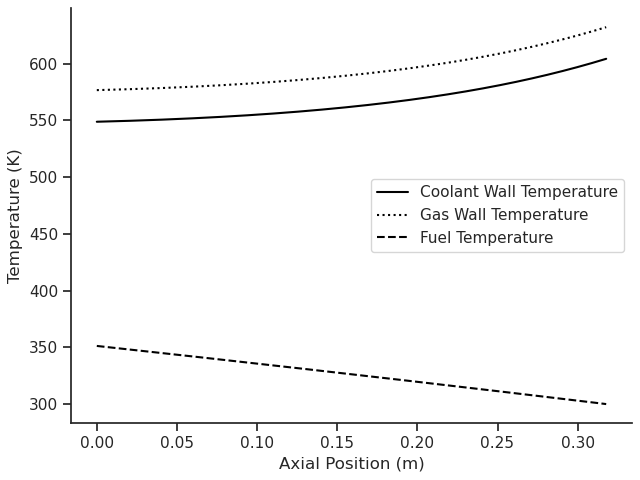
\includegraphics[width=0.8\linewidth]{Temperatures.png}
  \caption{Coolant and gas wall temperatures at 19\% of Bartz heat flux prediction.}
  \label{fig:temperatures}
\end{figure}

\begin{figure}[H]
  \centering
  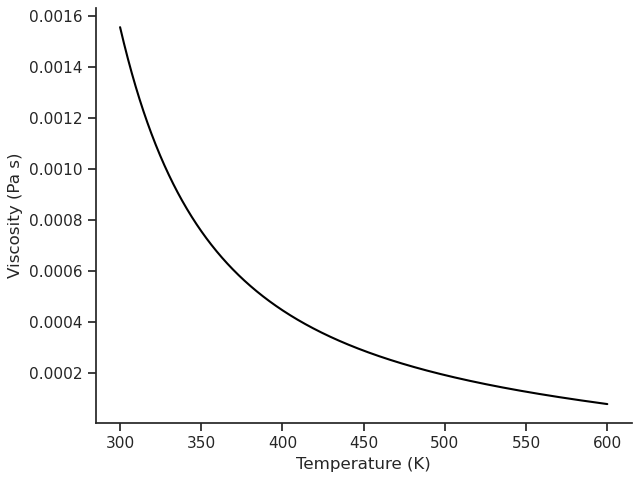
\includegraphics[width=0.8\linewidth]{Viscosity.png}
  \caption{RP-1 temperature dependence of viscosity.}
  \label{fig:viscosity}
\end{figure}

\printbibliography

\end{document}
